\section{多相催化反应过程中扩散影响的判定}


\begin{frame}
    \frametitle{外扩散影响的判定}
        \bigskip
        \begin{minipage}{0.48\linewidth}
            \begin{figure}[htpb]
                \centering
                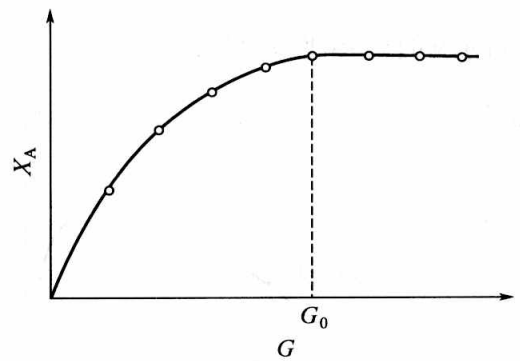
\includegraphics[width=\linewidth]{figures/fig6.8.png}
                \caption{流体质量速度对转化率的影响}
            \end{figure}            
        \end{minipage}\hfill
        \begin{minipage}{0.48\linewidth}
            \begin{itemize}
                \item 流体质量速度$G$，对外扩散有显著影响
                \item 保证在其他条件（如温度、反应物浓度、空时）相同的前提下，改变$G$以观察其对多相催化反应的影响。
                \item 当流体质量速度超过某一数值$G_0$时，外扩散对反应过程已无影响。
            \end{itemize}
        \end{minipage}

\end{frame}


\begin{frame}
    \frametitle{外扩散影响的判定}

    通过改变流体的质量速度以考察外扩散过程的影响，是多相催化反应动力学研究常采用的方法。实际生产的反应器难以采用上述方法。

    若能测得表观反应速率$\mathscr{R}_{\mathrm{A}}^{*}$，所进行的为$\alpha$级反应时，则可用下列判据来判定气相主体与催化剂外表面的浓度差是否可以忽略不计
    \[
        \frac{\mathscr{R}_{\mathrm{A}}^{*} L}{c_{\mathrm{AG}} k_{\mathrm{G}}}<\frac{0.15}{\alpha}
    \]
    气相与催化剂外表面间的温度差则可按下列判据来判断是否可以忽略
    \[
        \frac{L \mathscr{R}_{\mathrm{A}}^{*}\left(-\Delta H_{\mathrm{r}}\right)}{h_{\mathrm{S}} T_{\mathrm{G}}}<0.15 \frac{R T_{\mathrm{G}}}{E} 
    \]
    如符合上式，忽略相间温度差而造成反应速率的偏差不会大于5\%。

\end{frame}


\begin{frame}
    \frametitle{内扩散影响的判定}

    有效因子是梯尔模数的函数，当催化剂的组成和成型方法，以及反应的温度和反应物系的组成均一定时，仅取决于催化剂的颗粒粒度，因此，改变粒度进行实验，可以检验内扩散的影响程度。

    设所进行的是$\alpha$级不可逆反应，当外扩散影响已消除时，则其宏观反应速率可表示为
    \[
        \mathscr{R}_{\mathrm{A}}^{*}=-\frac{1}{W} \frac{\mathrm{d} N_{\mathrm{A}}}{\mathrm{d} t}=k_{\mathrm{W}} \eta c_\mathrm{AG}^ \alpha
    \]
    现有颗粒半径分别为$R_1$、$R_2$两种尺寸的同种催化剂床层，其反应条件维持相同，则反应速率之比为
    \[
        \frac{\mathscr{R}_{\mathrm{A} 1}^{*}}{\mathscr{R}_{\mathrm{A} 2}^{*}}=\frac{k_{\mathrm{W}} \eta_{1} c_{\mathrm{AG}}^{\alpha}}{k_{\mathrm{W}} \eta_{2} c_{\mathrm{AG}}^{\alpha}}=\frac{\eta_{1}}{\eta_{2}} 
    \]

\end{frame}


\begin{frame}
    \frametitle{内扩散影响的判定}

    \begin{itemize}
        \item 不存在内扩散影响时        
        \[
            \mathscr{R}_{\mathrm{A} 1} = \mathscr{R}_{\mathrm{A} 2}
        \]
        \item 内扩散影响严重时，反应速率与颗粒半径成反比。
        \[
            \frac{\mathscr{R}_{\mathrm{A} 1}^{*}}{\mathscr{R}_{\mathrm{A} 2}^{*}}=\frac{\eta_{1}}{\eta_{2}}=\frac{\phi_{2}}{\phi_{1}}=\frac{R_{2}}{R_{1}}
        \]        
    \end{itemize}
    一般情况下，反应速率总是随颗粒尺寸的增大而减小的，依此原理，在催化剂床层中装填同样形状但粒度不同的同一种催化剂，通入反应气体，在相同反应条件下测定其反应速率，检验内扩散的影响程度。

\end{frame}


\begin{frame}
    \frametitle{内扩散影响的判定}
    \begin{itemize}
        \item[1.] 粒度实验
    \end{itemize}
        \begin{minipage}{0.44\linewidth}
            \begin{figure}[htpb]
                \centering
                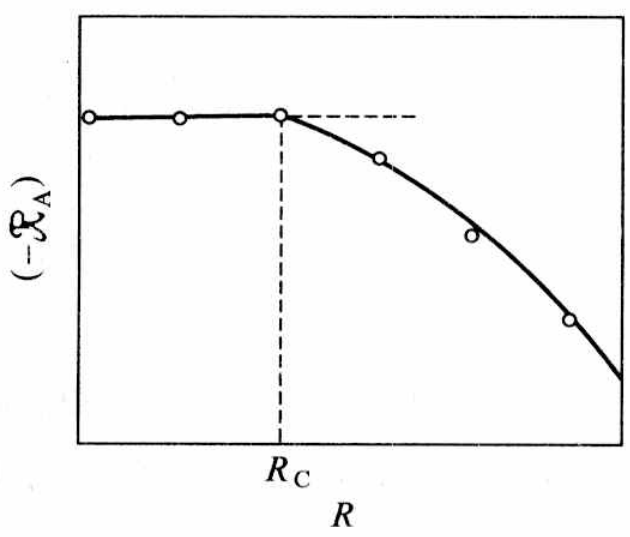
\includegraphics[width=\linewidth]{figures/fig6.9.png}
                \caption{催化剂半径对反应速率的影响}
            \end{figure}    
        \end{minipage}\hfill
        \begin{minipage}{0.48\linewidth}
            \begin{itemize}
                \item 反应速率将随粒度减小而增加。
                \item 当粒度减小到某一尺寸后，再减小粒度对反应速率即不再有影响
                \item 对$R<R_\mathrm{c}$的催化剂颗粒，内扩散阻力对反应过程可以认为没有影响。
                \item 内扩散不发生影响的粒度，与温度有关，也与浓度有关（一级反应例外）。
            \end{itemize}
        \end{minipage}

\end{frame}


\begin{frame}
    \frametitle{内扩散影响的判定}

    \begin{itemize}
        \item 反应温度越高，消除内扩散影响所要求的粒度越小。
        \item 浓度$c_{\mathrm{AS}}$越高，消除内扩散影响所要求的粒度越小。
    \end{itemize}

    对于$\alpha$级反应，
    \[
        \eta=\frac{\sqrt{2 D_{\mathrm{e}}}}{L \sqrt{k_{\mathrm{p}}} c_{\mathrm{AS}}^\alpha}\left[\int_{0}^{c_{\mathrm{AS}}} c_{\mathrm{A}}^\alpha \mathrm{d} c_{\mathrm{A}}\right]^{1 / 2}=\frac{1}{L} \sqrt{\frac{2 D_{\mathrm{e}}}{(\alpha+1) k_{\mathrm{p}} c_\mathrm{AS}^{\alpha - 1}}}
    \]
    为了要保持相同的$\eta$值，当浓度$c_{\mathrm{AS}}$增加时，催化剂的粒度$L$必须减小。    

    若在高温、高反应物浓度下，已判明消除了内、外扩散的影响。那么，可以保证在低温、低反应物浓度时也不会有内、外扩散的影响，反应物的级数为负数时为例外。

\end{frame}


\begin{frame}
    \frametitle{内扩散影响的判定}
    
    \begin{itemize}
        \item[2.] 测量表观反应速率$\mathscr{R}_{\mathrm{A}}^{*}$
    \end{itemize}
    

    若反应系统已排除外扩散阻力影响，对于一级反应，实测表观反应速率$\mathscr{R}_{\mathrm{A}}^{*}$为
    \[
        \mathscr{R}_{\mathrm{A}}^{*}=\eta k_{\mathrm{p}} c_{\mathrm{AG}}
    \]
    如果$k_{\mathrm{p}}$已知，显然可由上式求$\eta$来判断内扩散的影响程度。但是，在实际工业生产中，往往本征反应速率常数$k$和级数$n$是未知的，在这种情况下，可以通过计算无量纲参数$\phi^2\eta$来判断。$\mathscr{R}_{\mathrm{A}}^{*}=\eta k_{\mathrm{p}} c_{\mathrm{AG}}$代入$\phi = L\sqrt{\frac{k_\mathrm{p}}{D_{\mathrm{e}}}}$，得
    \[
        \phi=L \sqrt{\frac{\mathscr{R}_{\mathrm{A}}^{*}}{\eta c_{\mathrm{AG}}D_{\mathrm{e}}}}
    \]
    \[
        \phi^2\eta = \frac{L^2 \mathscr{R}_{\mathrm{A}}^{*}}{c_{\mathrm{AG}}D_{\mathrm{e}}}
    \]    

\end{frame}


\begin{frame}
    \frametitle{内扩散影响的判定}
    当催化剂具有不同颗粒形状时，
    \begin{itemize}
        \item 一般来说，$\phi \leqslant 0.4$时，$\eta \approx 1$，$\phi^2\eta <0.16$，表明内扩散阻力影响可忽略；
        \item $\phi \geqslant 3$时，$\eta \approx 1/\phi$，$\phi^2\eta \geqslant 3$，表明内扩散阻力有明显影响。
    \end{itemize}

    对于半径为$r_\mathrm{p}$的球形颗粒，
    \begin{itemize}
        \item $\phi^2\eta = \frac{r_\mathrm{p}^2 \mathscr{R}_{\mathrm{A}}^{*}}{c_{\mathrm{AG}}D_{\mathrm{e}}} \leqslant 1.4$时，可认为没有内扩散阻力影响；
        \item 当$\phi \geqslant 5$时，$\phi^2\eta = \frac{r_\mathrm{p}^2 \mathscr{R}_{\mathrm{A}}^{*}}{c_{\mathrm{AG}}D_{\mathrm{e}}} \geqslant 15$，表明内扩散阻力有明显影响。
    \end{itemize}
    为了改善颗粒内扩散阻力，可采取两个较为有效的措施：
    \begin{itemize}
        \item 在工程上能承受的压降条件下，尽可能地采用细颗粒催化剂。
        \item 改变催化剂的工程结构，降低内部传质阻力。
    \end{itemize}

\end{frame}

\begin{frame}
    \frametitle{内扩散影响的判定}

    上述结论是对一级反应导出的，亦可用于非一级反应，但$\phi$的定义要修改。
    
    定义一普遍化梯尔模数：
    \[
        \phi^{2}=\frac{L^{2} k_{\mathrm{p}}\left[f(c_{\mathrm{AG}})\right]^{2}}{2 D_{\mathrm{e}} \int_{c_{\mathrm{AC}}}^{c_{\mathrm{AG}}} f(c_{\mathrm{A}}) \mathrm{d} c_{\mathrm{A}}}
    \]
    \[
        \phi^{2} \eta=\frac{\mathscr{R}_{\mathrm{A}}^{*} L^{2} f(c_{\mathrm{AG}})}{2 D_{\mathrm{e}} \int_{c_{\mathrm{AC}}}^{c_{\mathrm{AG}}} f(c_{\mathrm{A}}) \mathrm{d} c_{\mathrm{A}}}
    \]

\end{frame}


\begin{frame}[t]
    \frametitle{}

    \begin{example}
        进行一气固相催化反应动力学的研究，反应为\ch{A + B -> R}，反应温度为200℃，A的分压$p_\mathrm{A} =\ $\SI{0.051}{MPa}，B的分压$p_\mathrm{B} =\ $\SI{0.253}{MPa}，B组分过量，该反应可看作一级反应。所用催化剂颗粒的平均直径为\SI{0.14}{cm}，催化剂颗粒密度为\SI{1.39}{g/cm^3}，测得表观反应速率$\mathscr{R} =$\SI{0.032}{mol/(h.g)}，若有效扩散系数$D_\mathrm{e} =$\SI{0.248}{cm^2/s}，试估计内部传递的影响。
    \end{example}\pause
    \vspace{-16pt}
    \[
        c_{\mathrm{AG}}=\frac{p_{\mathrm{A}}}{R T}=\frac{0.051}{8.314 \times 473}=1.29 \times 10^{-5} \mathrm{~mol} / \mathrm{cm}^{3}
    \]
    \[
        \mathscr{R}=\frac{0.032}{3600} \times 1.39=1.24 \times 10^{-5} \mathrm{~mol} /(\mathrm{s} \cdot \mathrm{cm}^{3})
    \]
    \[
        \Phi^{2} \eta=r_{\mathrm{p}}^{2} \frac{\mathscr{R}}{c_{\mathrm{AG}} D_{\mathrm{e}}}=0.07^{2} \frac{1.24 \times 10^{-5}}{1.29 \times 10^{-5} \times 0.0248}=0.19
    \]
    \[
        \Phi^{2} \eta=0.19<1.44 \qquad \text{内扩散阻力影响可忽略不计}
    \]

\end{frame}


